\documentclass[25pt, a0paper, portrait, margin=0mm, innermargin=0pt, blockverticalspace=0mm, colspace=0mm, subcolspace=0mm]{tikzposter} %Default values for poster format options.

%\tikzposterlatexaffectionproofon %shows small comment on how the poster was made at bottom of poster
\tikzposterlatexaffectionproofoff

\newcommand{\bmmax}{0}  
\newcommand{\hmmax}{0}  
\usepackage{amsmath}
\usepackage{amsfonts}
\usepackage{bbm}
\usepackage{bm}
\usepackage{scalerel}
\usepackage{sistyle}
\SIthousandsep{,}

\usepackage{booktabs} % For formal tables
\usepackage{multirow}
\usepackage{hyperref}

\usepackage{tikz}
\usetikzlibrary{arrows.meta}
\usetikzlibrary{backgrounds}
\usetikzlibrary{positioning, fit, mindmap, trees, calc,tikzmark,shapes}
\usetikzlibrary{shapes.arrows, fadings, automata,tikzmark,decorations.pathreplacing,patterns}

\usepackage{pgfplots}
\pgfplotsset{compat=1.8}

\usepackage[labelfont=bf]{caption}
\captionsetup{font=small}
\usepackage{float}
\usepackage{graphicx}
\usepackage{subfigure}
\usepackage{adjustbox}
\usepackage[inline]{enumitem}
\usepackage{fontawesome}

\usepackage[]{qrcode}

\usepackage{xcolor}

\definecolor{riptide}{RGB}{141,211,199}
\definecolor{pale_prim}{RGB}{255,255,179}
\definecolor{lavender_gray}{RGB}{190,186,218}
\definecolor{salmon}{RGB}{242,131,107}
\definecolor{seagull}{RGB}{128,177,211}
\definecolor{rajah}{RGB}{253,180,98}
\definecolor{yellow_green}{RGB}{198,222,119}
\definecolor{classic_rose}{RGB}{252,205,229}
\definecolor{feijoa}{RGB}{178,223,138}

\definecolor{cruise}{RGB}{179,226,205}
\definecolor{apricot}{RGB}{253,205,172}
\definecolor{periwinkle}{RGB}{203,213,232}
\definecolor{snow_flurry}{RGB}{230,245,201}
\definecolor{buttermilk}{RGB}{255,242,174}

\definecolor{sundown}{RGB}{249, 180, 181}
\definecolor{spindle}{RGB}{179,205,227}
\definecolor{tea_green}{RGB}{204,235,197}
\definecolor{languid_lavender}{RGB}{222,203,228}
\definecolor{champagne}{RGB}{254,217,166}
\definecolor{cream}{RGB}{255,255,204}


\definecolor{monte_carlo}{RGB}{135,204,194}
\definecolor{melon}{RGB}{254,191,181}
\definecolor{granny_smith_apple}{RGB}{150,214,150}
\definecolor{watusi}{RGB}{254,221,207}
\definecolor{see_green}{RGB}{161,228,195}

\definecolor{moss_green}{RGB}{170,216,176}
\definecolor{opal}{RGB}{164,207,190}

\definecolor{pale_turquoise}{RGB}{172,240,242}
\definecolor{Madang}{RGB}{190,235,159}
\definecolor{pixie_green}{RGB}{183,214,170}
\definecolor{coral_andy}{RGB}{243,204,205}
\definecolor{manhattan}{RGB}{226,180,125}
\definecolor{quartz}{RGB}{219,223,238}
\definecolor{spring_sun}{RGB}{242,243,195}
\definecolor{dairy_cream}{RGB}{254,226,189}
\definecolor{surf_crest}{RGB}{205,230,208}
\definecolor{french_pass}{RGB}{195,232,246}
\definecolor{cosmos}{RGB}{248,209,210}
\definecolor{portafino}{RGB}{245,237,160}
\definecolor{sail}{RGB}{163,205,235}
\definecolor{hint_green}{RGB}{226,246,209}


\definecolor{jet_stream}{RGB}{188, 214, 210}


\definecolor{azalea}{RGB}{251, 196, 196}
\definecolor{wewak}{RGB}{244, 143, 150}
\definecolor{bittersweet}{RGB}{255,111,105}
\definecolor{sunset_orange}{RGB}{242,89,75}
\definecolor{light_coral}{RGB}{244, 127, 123}
\definecolor{carnation}{RGB}{245, 80, 86}
\definecolor{flamingo}{RGB}{237, 88, 85}
\definecolor{carmine_pink}{RGB}{231, 76, 60}
\definecolor{deep_carmine_pink}{RGB}{236, 50, 67}
\definecolor{fire_engine_red}{RGB}{210,44,41}
\definecolor{amaranth}{RGB}{234,46,73}
\definecolor{ku_crimson}{RGB}{243, 0, 25}
\definecolor{fire_engine_red}{RGB}{206, 37, 51}
\definecolor{copper_rust}{RGB}{155, 64, 74}

\definecolor{chilean_fire}{RGB}{215, 87, 44}

\definecolor{japanese_laurel}{RGB}{53, 116, 40}


\definecolor{turmeric}{RGB}{211, 178, 76}
\definecolor{saffron}{RGB}{249,193,62}
\definecolor{my_sin}{RGB}{255, 176, 59}
\definecolor{tree_poppy}{RGB}{246, 154, 27}
\definecolor{jaffa}{RGB}{240, 131, 58}
\definecolor{crusta}{RGB}{254, 127, 44}
\definecolor{tahiti_gold}{RGB}{223, 102, 36}
\definecolor{outrageous_orange}{RGB}{255, 100, 45}
\definecolor{safety_orange}{RGB}{254, 106, 0}



\definecolor{turquoise}{RGB}{41,217,194}
\definecolor{puerto_rico}{RGB}{94, 194, 166}
\definecolor{mountain_meadow}{RGB}{0, 163, 136}
\definecolor{free_speech_aquamarine}{RGB}{0, 156, 114}
\definecolor{java}{RGB}{2,190,196}


% person:
\definecolor{matisse}{RGB}{25, 104, 167}
\definecolor{shakespeare}{RGB}{85, 154, 193}
\definecolor{mona_lisa}{RGB}{246,152,134}

% gray:
\definecolor{bgc}{RGB}{245,245,245}
\definecolor{tuatara}{RGB}{67, 67, 67}
\definecolor{aluminum}{RGB}{153,153,153}
\definecolor{silver}{RGB}{191,191,191}
\definecolor{platinum}{RGB}{228,228,228}
\definecolor{mercury}{RGB}{230,230,230}
\definecolor{gallery}{RGB}{240,240,240}
\definecolor{athens_gray}{RGB}{236, 240, 241}
\definecolor{ship_gray}{RGB}{77,77,77}


% nature color
\definecolor{early_dawn}{RGB}{252,243,218}
\definecolor{egg_shell}{RGB}{238, 234, 215}
\definecolor{midnight}{RGB}{0, 29, 50}
\definecolor{sundown}{RGB}{249, 180, 181}
\definecolor{sun_shade}{RGB}{255, 144, 68}
\definecolor{sushi}{RGB}{117, 168, 47}
\definecolor{tomato}{RGB}{255, 97, 56}
\definecolor{ice_cold}{RGB}{169,232,220}


% blue:
\definecolor{regal_blue}{RGB}{5,63,114}
\definecolor{jelly_bean}{RGB}{45, 126, 150}
\definecolor{celestial_blue}{RGB}{52, 152, 219}
\definecolor{curious_blue}{RGB}{41, 128, 185}
\definecolor{french_blue}{RGB}{0, 112, 182}
\definecolor{matisse}{RGB}{25, 104, 167}

\definecolor{biscay}{RGB}{44, 62, 80}

% green:
\definecolor{cosmic_latte}{RGB}{222, 247, 229}
\definecolor{chinook}{RGB}{163, 232, 178}
\definecolor{padua}{RGB}{121, 189, 143}
\definecolor{ocean_green}{RGB}{79, 176, 112}
\definecolor{pastel_green}{RGB}{107, 227, 135}
\definecolor{chateau_green}{RGB}{69, 191, 85}
\definecolor{RoyalBlue}{RGB}{69, 191, 85}
\definecolor{pigment_green}{RGB}{0, 175, 79}
\definecolor{fern}{RGB}{101,197,117}
\definecolor{killarney}{RGB}{56, 113, 66}
\definecolor{viridian}{RGB}{70, 137, 102}


\definecolor{dark_burgundy}{RGB}{123,19,8}
\definecolor{outrageous_orange}{RGB}{251,102,46}



\geometry{paperheight=120cm, paperwidth=80cm}

\renewcommand{\familydefault}{\sfdefault}
\newcommand\NameBlock[1]{\node[fit=(blockbody)(blocktitle),inner sep=-5pt] (#1) {};}

\settitle{ \centering \vbox{
\color{black} {\bfseries \Huge \@title \par}
\@titlegraphic \\
[\TP@titlegraphictotitledistance] \centering 
%\vspace*{0.5cm}
{\color{gray} \huge \@author \par} 
%\vspace*{1em} 
{\LARGE \@institute}
}}


% Commands
\newcommand{\bs}{\textbackslash}   % backslash
\newcommand{\cmd}[1]{{\bf \color{red}#1}}   % highlights command

% Title, Author, Institute
%\title{\parbox{1\linewidth}{\centering BERT4Rec: Sequential Recommendation with Bidirectional Encoder Representations from Transformer}}
%\author{Fei Sun, Jun Liu, Jian Wu, Changhua Pei, Xiao Lin, Wenwu Ou, and Peng Jiang}
%\institute{\parbox{\linewidth}{\centering Alibaba Group\\
%%\texttt{ofey.sunfei@gmail.com, \{guojiafeng, lanyanyan,\hspace{-4mm} junxu,\hspace{-4mm} cxq\}@ict.ac.cn\}}
%}
%}
%\titlegraphic{
%\hspace{-8cm}
%\includegraphics[width=1.2\linewidth]{top_deco.png}
%\hspace{cm}
%
\includegraphics[width=7cm,height=7cm]{cas.pdf}
%\hspace{5.5cm}
%\hfill
%}

%\titlegraphic{\qrcode[hyperlink,height=2in]{http://ofey.me/projects/wordrep/}}
% -- PREDEFINED THEMES ---------------------- %
% Choose LAYOUT:  Default, Basic, Rays, Simple, Envelope, Wave, Board, Autumn, Desert,
\usetheme{Simple}
\colorlet{notebgcolor}{flamingo}
\colorlet{noteframecolor}{flamingo}
\colorlet{backgroundcolor}{white}
\colorlet{titlefgcolor}{white}
\colorlet{titlebgcolor}{white}

%\defineblockstyle{MyBlock}{% define a custom style for a block
%    titlewidthscale=0.8, bodywidthscale=1, titlecenter,
%    titleoffsetx=0pt, titleoffsety=0pt, bodyoffsetx=0pt, bodyoffsety=15mm,
%    bodyverticalshift=15mm, roundedcorners=22, linewidth=5pt,
%    titleinnersep=8mm, bodyinnersep=8mm
%}{
%    \draw[rounded corners=\blockroundedcorners, inner sep=\blockbodyinnersep,
%          line width=0pt, color=white,
%          top color=white, bottom color=white,
%          %fill=blockbodybgcolor
%          ]
%      (blockbody.south west) rectangle (blockbody.north east); %
%}
%\newcommand\myblock[3][MyBlock]{\useblockstyle{#1}\block{#2}{#3}}



\begin{document}
\useblockstyle{Basic}

\maketitle[titletotopverticalspace=0cm, width=\linewidth, roundedcorners=0, linewidth=0pt,titletoblockverticalspace=0cm]

%https://tex.stackexchange.com/questions/413936/tikzposter-without-maketitle
\makeatletter
    \setlength{\TP@blocktop}{.5\textheight}
\makeatother
    
\colorlet{blockbodybgcolor}{regal_blue}
\block[linewidth=0pt, roundedcorners=0, bodyinnersep=15mm]{}{
\color{white}
\centering
\begin{minipage}{0.8\linewidth}
    \fontsize{70}{100} \selectfont
Instead of left-to-right \textbf{unidirectional model} \&  \textbf{predicting next}%\& \textbf{next item prediction}
\begin{center}
    
\includegraphics[scale=2]{uni}
\end{center}
\vspace*{-0.5cm}
we use \textbf{bidirectional self-attention model} \& \textbf{cloze task}
\begin{center}
    
\includegraphics[scale=1.8]{model}
\end{center}
\vspace*{-0.5cm}
for representation learning in \textbf{sequential recommendation} 
\end{minipage}

\large ~~ 

\large ~~ 

}\NameBlock{main}

\colorlet{blockbodybgcolor}{white}
\begin{columns} %blocks will be placed into columns
    \column{.7}
    
    \block[linewidth=0pt, roundedcorners=0, bodyinnersep=15mm]{}{

\parbox{\linewidth}{\centering \bfseries \huge \color{outrageous_orange} BERT4Rec: Sequential Recommendation with Bidirectional Encoder Representations from Transformer}
\parbox{\linewidth}{\tiny ~~\\}
\parbox{\linewidth}{\centering \color{outrageous_orange} \Large Fei Sun, Jun Liu, Jian Wu, Changhua Pei, Xiao Lin, Wenwu Ou, and Peng Jiang}

}

     \begin{subcolumns}
        \subcolumn{.5}
        \block[linewidth=0pt, bodyverticalshift=-0.5cm]{}{
        \centering
        \hspace*{3.6cm}\begin{minipage}{0.9\linewidth}
           {\Large \textbf{Motivation}}
        \vspace*{0.5cm}
        \begin{equation*}
            p\bigl(v_{n_u+1}^{(u)}=v|\ \mathcal{S}_u\bigr), \,\,\mathcal{S}_u{=}[v_1^{(u)},\dots,v_t^{(u)},\dots,v_{n_u}^{(u)}]
        \end{equation*}
        \vfill
        \begin{itemize} [leftmargin=2cm]
            \item Unidirectional models restrict the power of hidden representations for items in the historical sequences.
            \item Rigid order assumption in unidirectional sequential models is not always right in user behavior sequences.
            \item User behaviors are often noisy due to a variety of unobservable external factors. They usually are roughly chronological, but not rigidly ordered.
        \end{itemize} 
        \end{minipage}
        }
        
        \block[linewidth=0pt, bodyverticalshift=-0.cm]{}{

        \hspace*{3.6cm}\begin{minipage}{0.9\linewidth}
           {\Large \textbf{Model}}
        
        \begin{center}
        \begin{adjustbox}{max width=1.05\linewidth}
        \begin{tabular}{ c c}
        \raisebox{-.5\height}{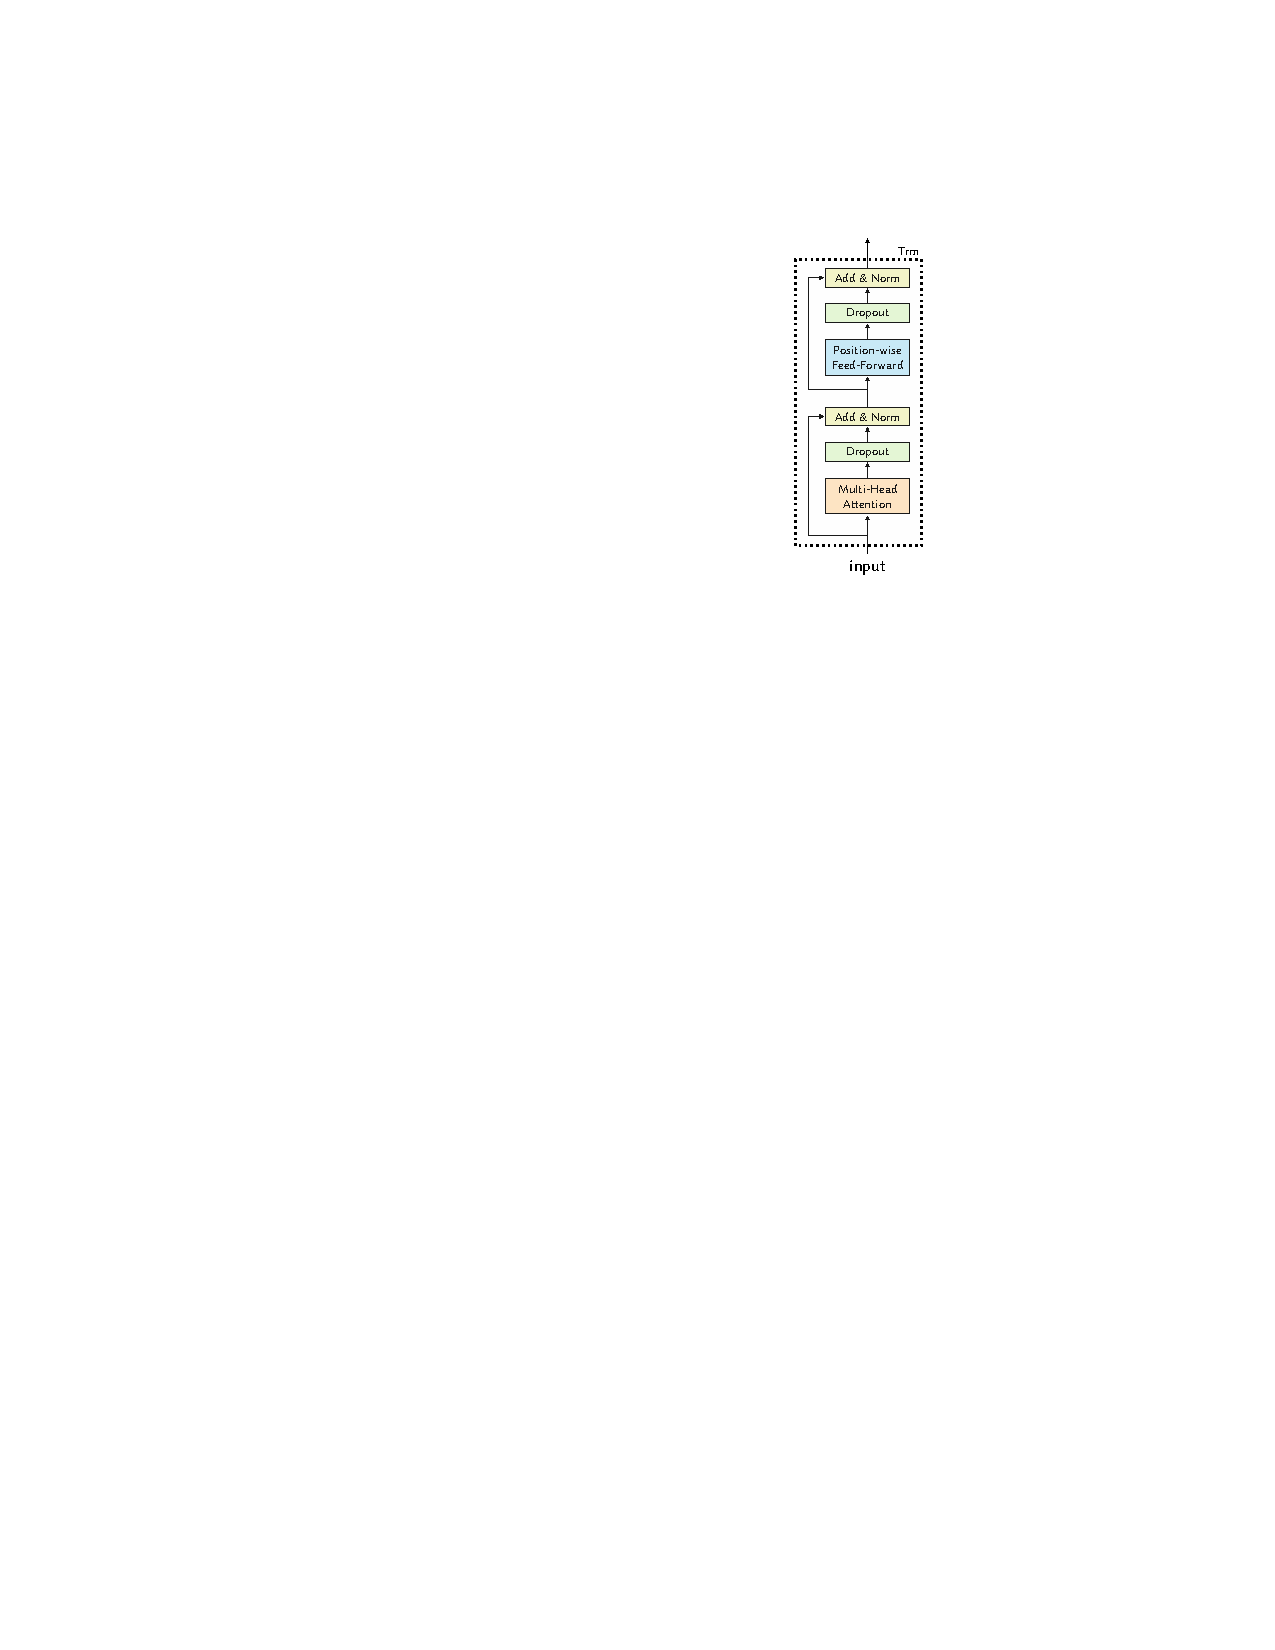
\includegraphics[scale=2.4]{trm}}~ & \normalsize $\begin{aligned}
        \mathtt{Att}(\bm{Q},\!\bm{K},\!\bm{V}) &= \mathrm{softmax} \biggl(\frac{\bm{Q}\bm{K}^{\top}}{\sqrt{d/h}}\biggr) \bm{V}\\
        \text{head}_i &= \mathtt{Att}\bigl(\bm{H}^l\bm{W}_i^Q, \bm{H}^l\bm{W}_i^K, \bm{H}^l\bm{W}_i^V \bigr)\\
            \mathtt{MH}(\bm{H}^{l}) &= [\text{head}_1; \text{head}_2; \dots; \text{head}_h]\bm{W}^{O} \\
        \mathtt{FFN}(\bm{x}) &= \texttt{GELU}\bigl(\bm{x} \bm{W}^{(1)}+\bm{b}^{(1)}\bigr)\bm{W}^{(2)} + \bm{b}^{(2)}\\
        \texttt{GELU}(x) &= x \Phi(x), {\color{gray}\Phi(x)\text{ is CDF of standard normal}}\\
        \texttt{PFFN}(\bm{H}^l) & = \bigl[\mathtt{FFN}(\bm{h}_1^{l})^{\top}; \dots; \mathtt{FFN}(\bm{h}_t^{l})^{\top}\bigr]^{\top}\\
        \bm{A}^{l-1} &= \mathtt{LN}\Bigr(\bm{H}^{l-1} + \mathtt{Dropout}\bigl(\mathtt{MH}(\bm{H}^{l-1})\bigr)\Bigr) \\
        \mathtt{Trm}(\bm{H}^{l-1}) &= \mathtt{LN}\Bigl(\bm{A}^{l-1} +  \mathtt{Dropout}\bigl(\mathtt{PFFN}(\bm{A}^{l-1})\bigr)\Bigr) \\
        \bm{H}^l &= \mathtt{Trm}\bigl(\bm{H}^{l-1}\bigr), \quad \forall i \in [1,\dots, L] \\
        \bm{h}_{i}^0 &= \bm{v}_i + \bm{p}_i
        \end{aligned}$
        \end{tabular}
        \end{adjustbox}
        \end{center}

        \end{minipage}
        }
        
        \block[linewidth=0pt]{}{
        \centering
        \hspace*{3.6cm} \begin{minipage}{0.9\linewidth}
          {\Large \textbf{Learning}~~ {\color{gray} \textit{cloze} task/random item mask}}\\
        {\small ~~}
        
        \centering
        \normalsize
        \renewcommand{\arraystretch}{1.6}
        \begin{adjustbox}{max width=\textwidth}
        \begin{tabular}{r c}
        \textbf{Samples}:~~~ & \raisebox{-.45\height}{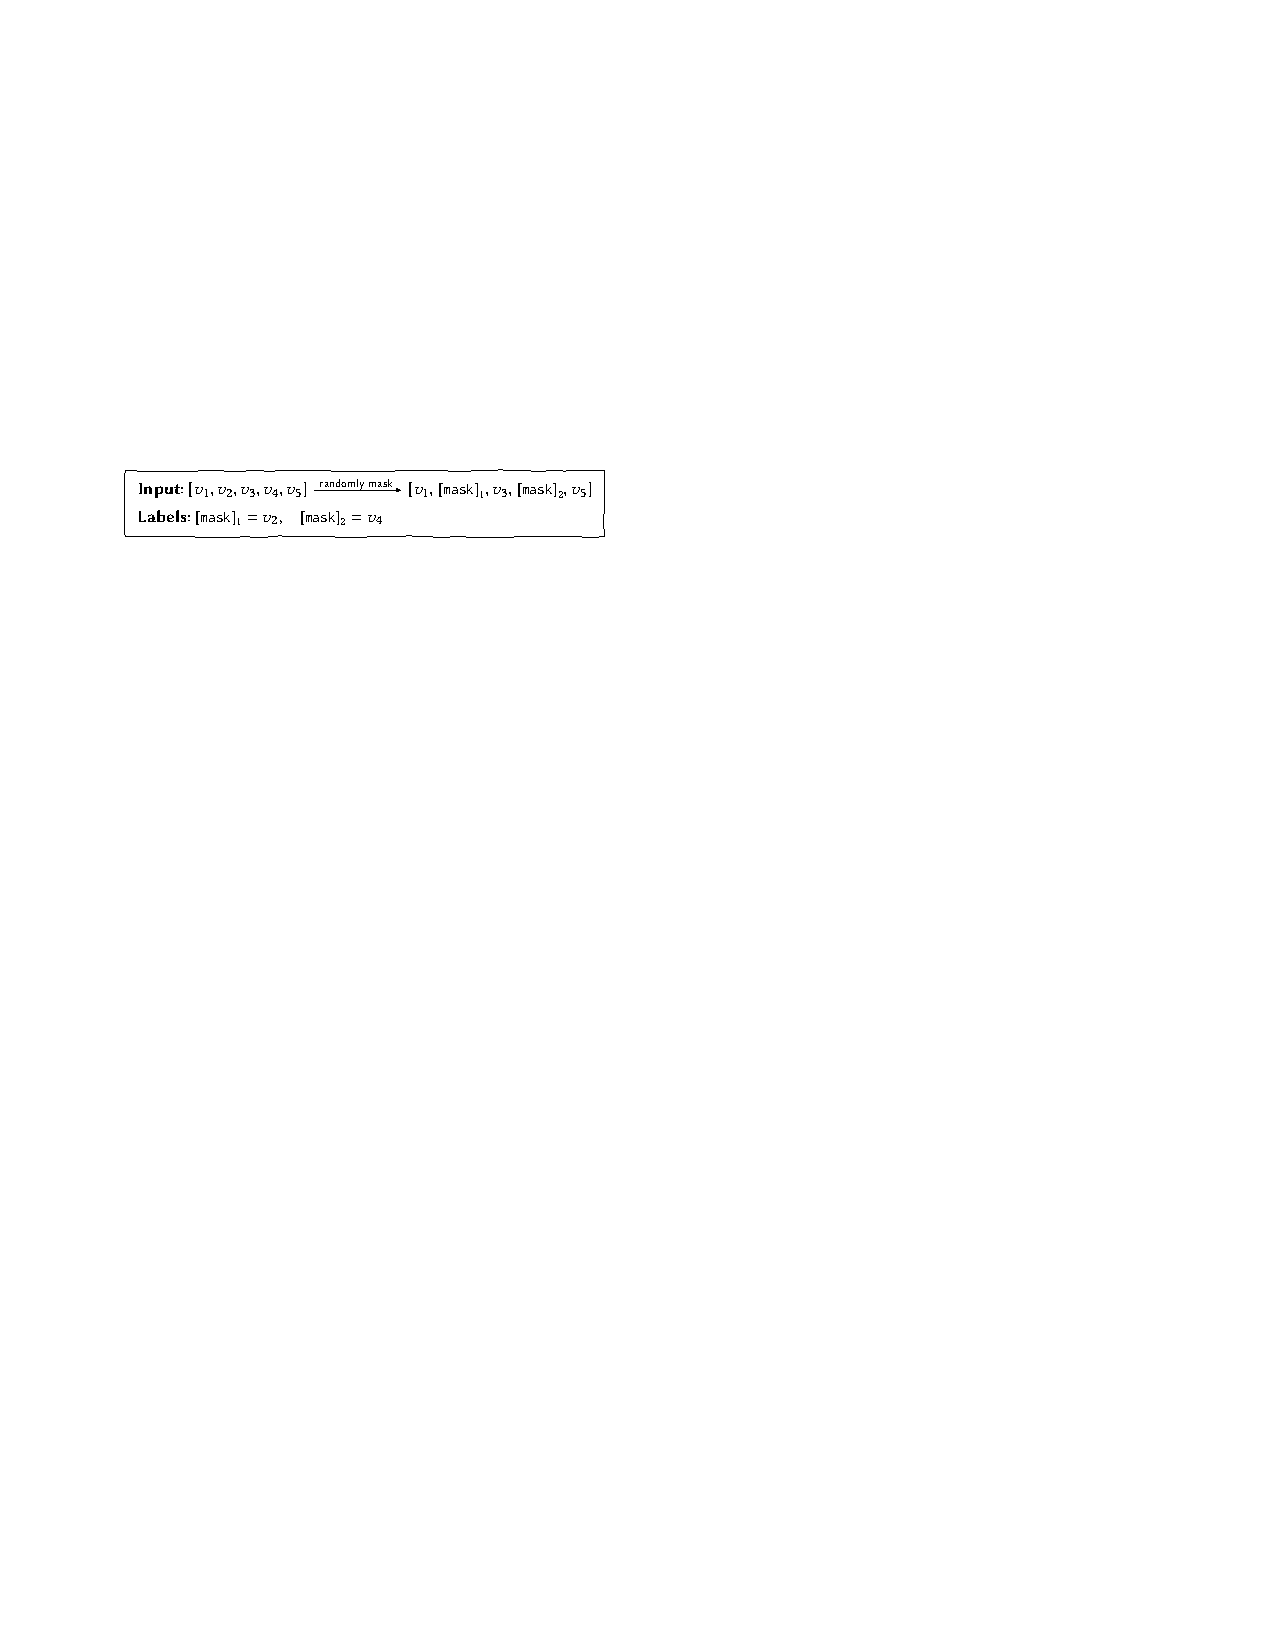
\includegraphics[scale=2]{sample}} \\
        \multirow{2}{*}{\textbf{Training}:}~~~ & $
            \mathcal{L} = \frac{1}{|\mathcal{S}_u^m|} \displaystyle \sum_{v_m\in \mathcal{S}_u^m} -\log P(v_m=v_m^{*}|\mathcal{S}_u^{\prime} )$ \\
        & \small \color{gray} $P(v) = \mathrm{softmax}\bigl(\mathtt{GELU}(\bm{h}_t^L \bm{W}^P +\bm{b}^P) \bm{E}^{\top} + \bm{b}^O \bigr)$\\
            \textbf{Predicting}:~~~ & $\mathcal{S}_u$.\texttt{append}(``\texttt{[mask]}'')  \& predict 
        \end{tabular}
        \end{adjustbox}
        
        \end{minipage}
        }
        

        \subcolumn{.5}
        
        \block[linewidth=0pt, bodyverticalshift=-0.5cm]{}{
                \centering
        \begin{minipage}{0.9\linewidth}
            {\Large \textbf{Experiments} }
        \vspace*{0.5cm}
        
        \normalsize
        \textbf{Datasets}
           \begin{center}
            \begin{adjustbox}{max width=0.95\linewidth}
            \setlength{\tabcolsep}{0.62em}
            \begin{tabular}{l r r r r r}
            \toprule
            Datasets & \#users & \#items & \#actions & Avg. length &  Density\\
            \midrule
            \textbf{Beauty} & \num{40226} & \num{54542} & 0.35m & 8.8 & 0.02\% \\
            \textbf{Steam} & \num{281428} & \num{13044} & 3.5m & 12.4 & 0.10\% \\
            \textbf{ML-1m} & \num{6040} & \num{3416} & 1.0m & 163.5 & 4.79\% \\
            \textbf{ML-20m} & \num{138493} & \num{26744} & 20m & 144.4 & 0.54\%\\
            \bottomrule
            \end{tabular}
            \end{adjustbox}
            \end{center}
            
        \vspace*{0.5cm}
        \textbf{Task Settings \& Evaluation Metrics \& Baselines}
        
        \begin{center}
        \begin{adjustbox}{max width=0.95\linewidth}
        \renewcommand{\arraystretch}{1.5}
        \begin{tabular}{l c l}
            Protocal & Metrics & Baselines \\ \toprule
           \multirow{2}{*}{\shortstack[l]{\textit{leave-one-out} evaluation: $S_u=[v_1^{(u)},\dots,v_{n_u}^{(u)}]$\\ train: $[v_1^{(u)},\dots,v_{n_u-2}^{(u)}]$, val: $v_{n_u-1}^{u}$, test: $v_{n_u}^{u}$ }} & 
           \multirow{4}{*}{\small $\begin{aligned}\mathrm{HR}@k &= \frac{1}{\vert \mathcal{U} \vert}\sum_{u \in \mathcal{U}} \mathbbm{1}(\mathrm{R}_{u, g_u} \leq k)\\
                \mathrm{NDCG}@k &= \frac{1}{\vert \mathcal{U} \vert}\sum_{u \in \mathcal{U}} \frac{2^{\mathbbm{1}(\mathrm{R}_{u, g_u} \leq k)} - 1}{\log_2 (\mathrm{R}_{u, g_u} + 1)}\\
                \mathrm{MRR} &= \frac{1}{\vert \mathcal{U} \vert}\sum_{u \in \mathcal{U}}\frac{1}{\mathrm{R}_{u, g_u}}
                 \end{aligned}$ }
                  & GRU4Rec \\
         &  & Caser \\ \cmidrule{1-1}
         \multirow{2}{*}{\shortstack[l]{Picking up the ground truth item from 100 \\ \vspace{0.1cm} \\ randomly sampled (by spopularity) negative items}} &  & GRU4Rec$^{+}$ \\
          &  & SASRec \\
        \end{tabular}
        \end{adjustbox}
        \end{center}
        
        \vspace*{0.3cm}
        \normalsize
        \textbf{Overall Performances}
        \begin{center}
        \begin{adjustbox}{max width=0.95\textwidth}
        \begin{tabular}{l l c c c c c c}
        \toprule
        Datasets & Metric &  GRU4Rec & GRU4Rec$^+$ & Caser & SASRec & BERT4Rec & Improv.\\
        \midrule
         \multirow{5}{*}{Beauty} & HR@5  & 0.1315 & 0.1781 & 0.1625 & \underline{0.1934} & \textbf{0.2207} & 14.12\%\\
         & HR@10 & 0.2343 & 0.2654 & 0.2590 & \underline{0.2653} & \textbf{0.3025} & 14.02\%\\
         & NDCG@5 & 0.0812 & 0.1172 & 0.1050 & \underline{0.1436} & \textbf{0.1599} & 11.35\%\\
         & NDCG@10  & 0.1074 & 0.1453 & 0.1360 & \underline{0.1633} & \textbf{0.1862} & 14.02\%\\
          & MRR & 0.1023 & 0.1299 & 0.1205 & \underline{0.1536} & \textbf{0.1701} & 10.74\%\\
         \midrule
         \multirow{5}{*}{Steam} & HR@5 & 0.2171 & 0.2391 & 0.1766 & \underline{0.2559} & \textbf{0.2710} & ~~5.90\%\\
         & HR@10  & 0.3313 & 0.3594 & 0.2870 & \underline{0.3783} & \textbf{0.4013} & ~~6.08\% \\
         & NDCG@5 & 0.1370 & 0.1613 & 0.1131 & \underline{0.1727} & \textbf{0.1842} & ~~6.66\% \\
         & NDCG@10 & 0.1802 & 0.2053 & 0.1484 & \underline{0.2147} & \textbf{0.2261} & ~~5.31\%\\
         & MRR & 0.1420 & 0.1757 & 0.1305 & \underline{0.1874} & \textbf{0.1949} & ~~4.00\%\\
         \midrule
         \multirow{5}{*}{ML-1m} & HR@5 & 0.4673 & 0.5103 & 0.5353 & \underline{0.5434} & \textbf{0.5876} & ~~8.13\%\\
         & HR@10 & 0.6207 & 0.6351 &  \underline{0.6692} & 0.6629 & \textbf{0.6970} & ~~4.15\%\\
         & NDCG@5 & 0.3196 & 0.3705 & 0.3832 & \underline{0.3980} & \textbf{0.4454} & 11.91\%\\
         & NDCG@10  & 0.3627 & 	0.4064 & 0.4268 & \underline{0.4368} & \textbf{0.4818} & 10.32\%\\
         & MRR & 0.3041 & 	0.3462 & 0.3648 & \underline{0.3790} & \textbf{0.4254} & 12.24\%\\
         \midrule
         \multirow{5}{*}{ML-20m} & HR@5  & 0.4657 & 0.5118 & 0.3804 & \underline{0.5727} & \textbf{0.6323} & 10.41\%\\
         & HR@10 & 0.5844 & 0.6524 & 0.5427 & \underline{0.7136} & \textbf{0.7473} & ~~4.72\% \\
         & NDCG@5 & 0.3090 & 0.3630 & 0.2538 & \underline{0.4208} & \textbf{0.4967} & 18.04\%\\
         & NDCG@10 & 0.3637 & 	0.4087 & 0.3062 & \underline{0.4665} & \textbf{0.5340} & 14.47\% \\
         & MRR & 0.2967 & 0.3476 & 0.2529 & \underline{0.4026} & \textbf{0.4785} & 18.85\% \\
        \bottomrule
        \end{tabular}
        \end{adjustbox}
        \end{center}
        
        \vspace*{0.5cm}
        \normalsize
        \textbf{Effectiveness of bidirectional self-attention \& Cloze objective}
        \begin{center}
            \begin{adjustbox}{max width=0.95\linewidth}
    \begin{tabular}
        {l c c c c c c}
        \toprule
       \multirow{2}{*}{Model} & \multicolumn{3}{c}{Beauty} & \multicolumn{3}{c}{ML-1m} \\ \cmidrule(lr){2-4} \cmidrule(lr){5-7}
        & HR@10 & NDCG@10 & MRR & HR@10 & NDCG@10 & MRR \\ \midrule
        SASRec & 0.2653 & 0.1633 & 0.1536 & 0.6629 & 0.4368 & 0.3790 \\
        BERT4Rec (1 mask) & 0.2940 & 0.1769 & 0.1618 & 0.6869 & 0.4696 & 0.4127 \\
        BERT4Rec & 0.3025 & 0.1862 & 0.1701 & 0.6970 & 0.4818 & 0.4254 \\ 
        \bottomrule
    \end{tabular}
    \end{adjustbox}
        \end{center}
    
        \end{minipage}
        }
    \end{subcolumns}
    
    % bodyverticalshift=-1cm
    \block[linewidth=0pt, bodyverticalshift=-0.3cm]{}{
    
%    \begin{minipage}{0.9\linewidth}
%    
%    \end{minipage}

    \begin{center}
        \begin{tabular}{l c}
        \shortstack[l]{\large \textbf{Impact of hidden} \\ \textbf{dimensionality $d$} }  & \raisebox{-.5\height}{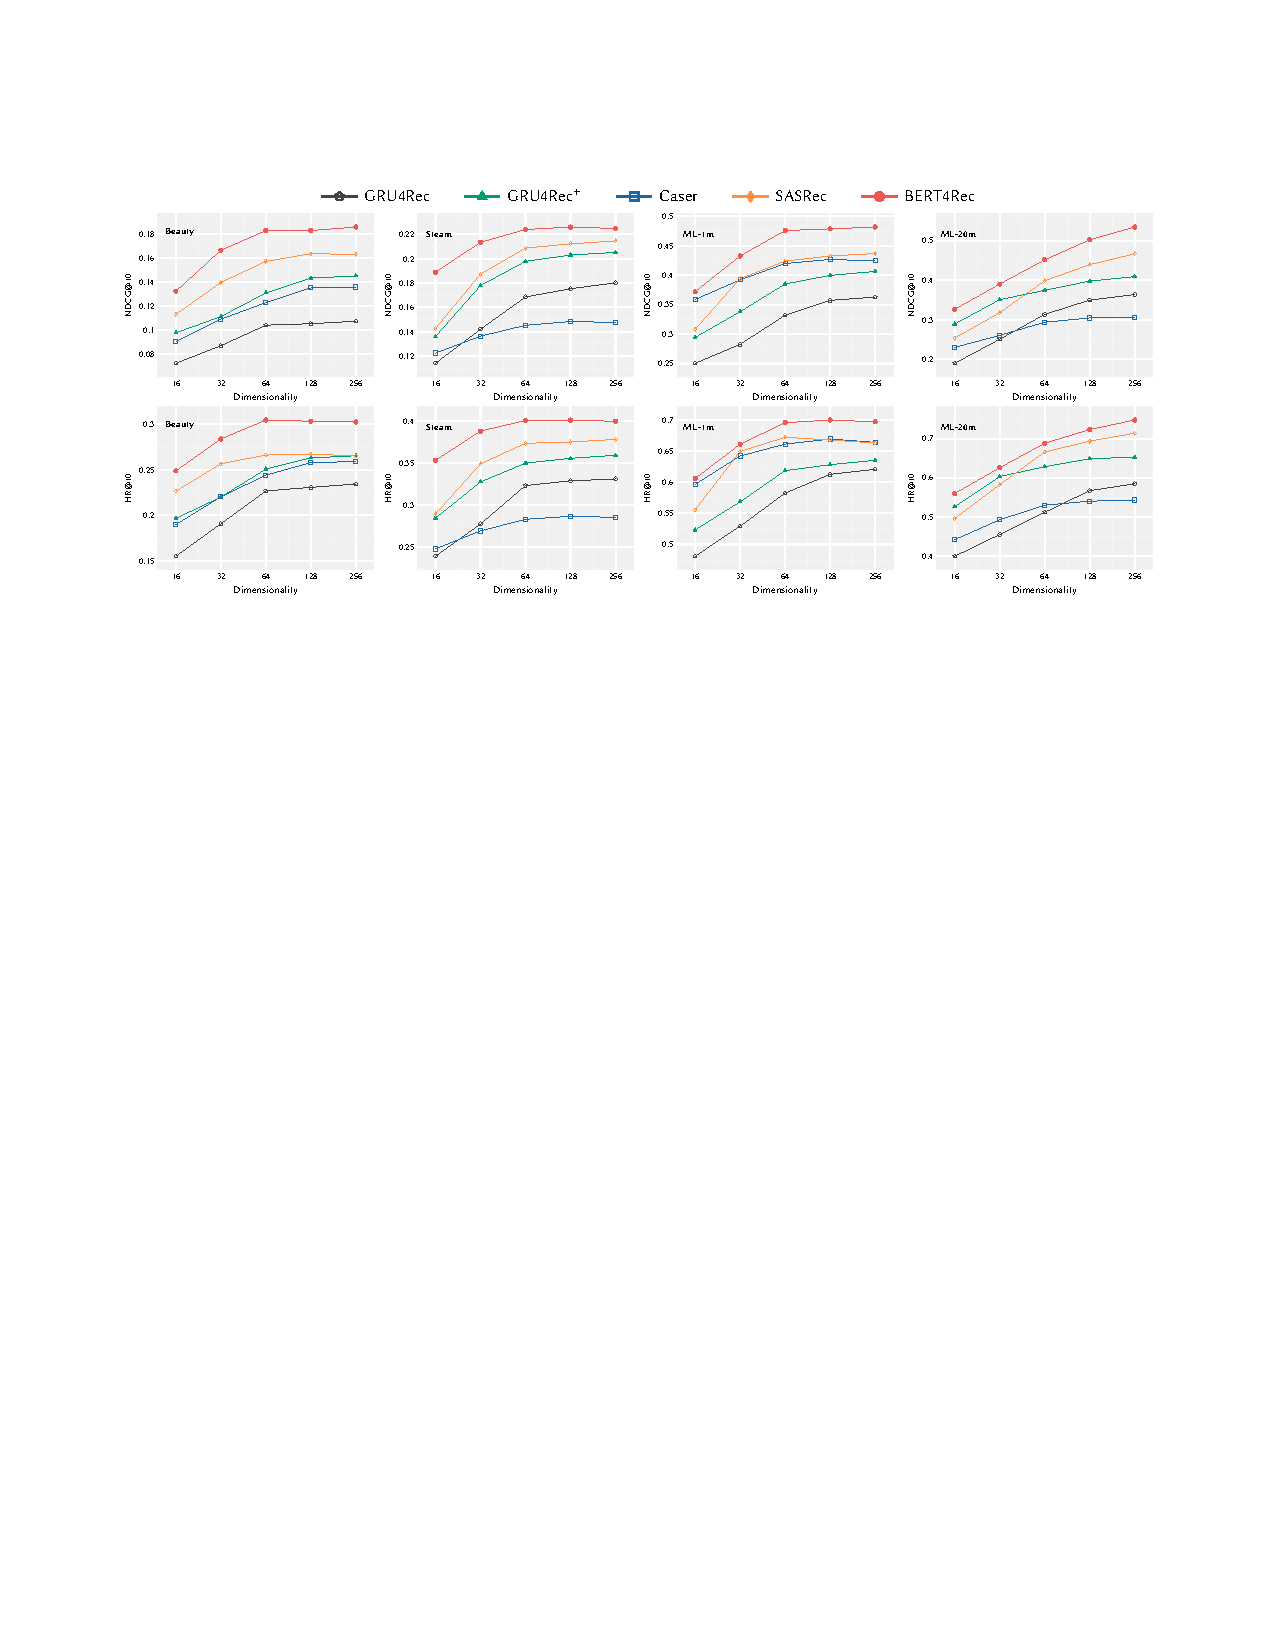
\includegraphics[scale=2.2]{exp_dim} }
        \end{tabular}
    \end{center}
    
    }

    \column{.3}

    \block[linewidth=0pt, roundedcorners=0, bodyinnersep=15mm, bodyoffsetx=-2.5cm]{}{
    \centering
        \begin{minipage}{0.9\linewidth}
            {\huge \textbf{Extra Results} }
        \end{minipage}
        }

%    \note[targetoffsetx=-.04\textwidth, targetoffsety=-7cm,innersep=0pt,angle=-45, radius=6cm, width=6.5cm]{\small Negative Sampling}
    \block[linewidth=0pt, roundedcorners=0, bodyinnersep=15mm, bodyoffsetx=-2.5cm, bodyverticalshift=0.7cm]{}{
    \centering
        \begin{minipage}{0.9\linewidth}
            {\Large \textbf{Impact of Mask Proportion $\rho$} }
        \vspace*{0.5cm}
        
        \begin{tikzfigure}
            \centering
             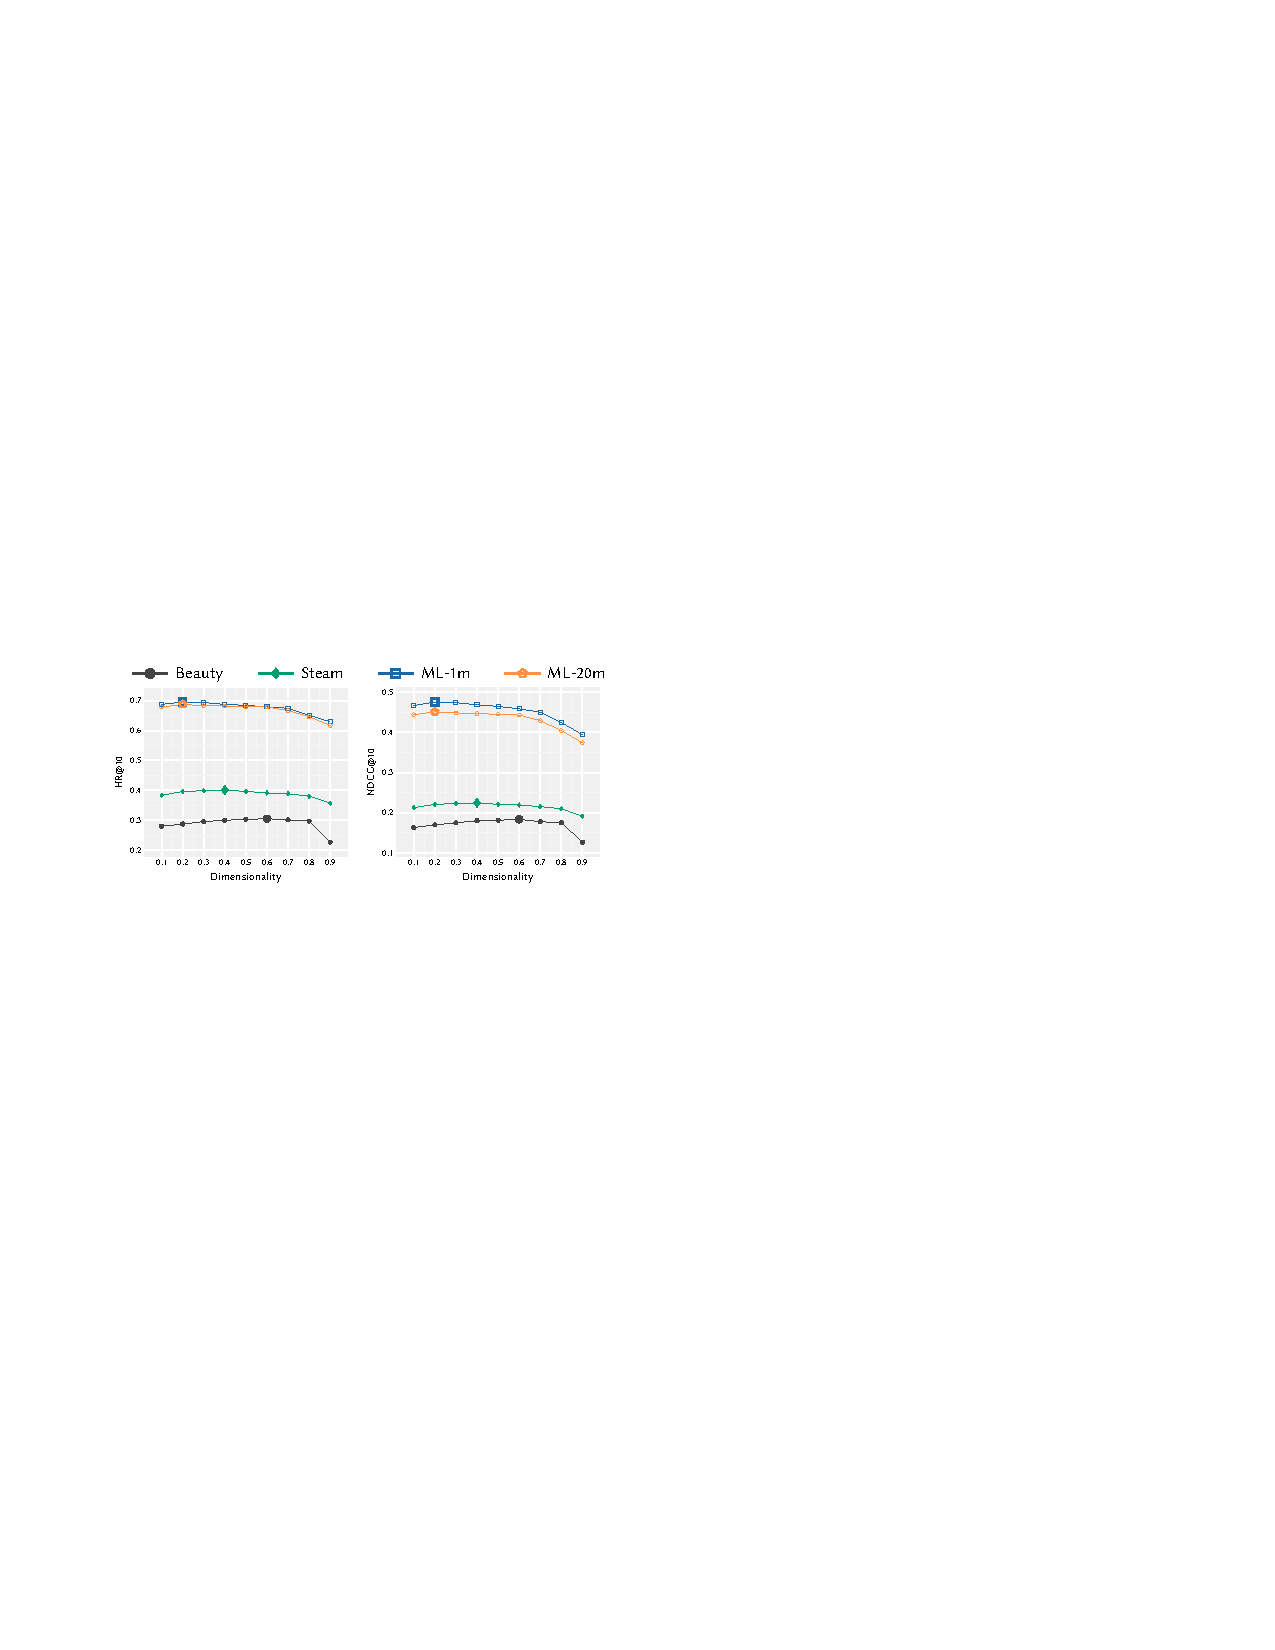
\includegraphics[scale=2.4]{mask_proportion}
        \end{tikzfigure}
        \centering
        \parbox{0.9\linewidth}{\bfseries \small Performance with different mask proportion $\rho$ on $d=64$. Bold symbols denote the best scores in each line.}
        \end{minipage}
    }

    \block[linewidth=0pt, roundedcorners=0, bodyinnersep=15mm, bodyoffsetx=-2.5cm, bodyverticalshift=-0.7cm]{}{
        \centering
        \begin{minipage}{0.9\linewidth}
            {\Large \textbf{Attention Visualization} }
            
            \vspace*{0.5cm}
            \begin{tikzfigure}
            
            \begin{minipage}{0.45\textwidth}
            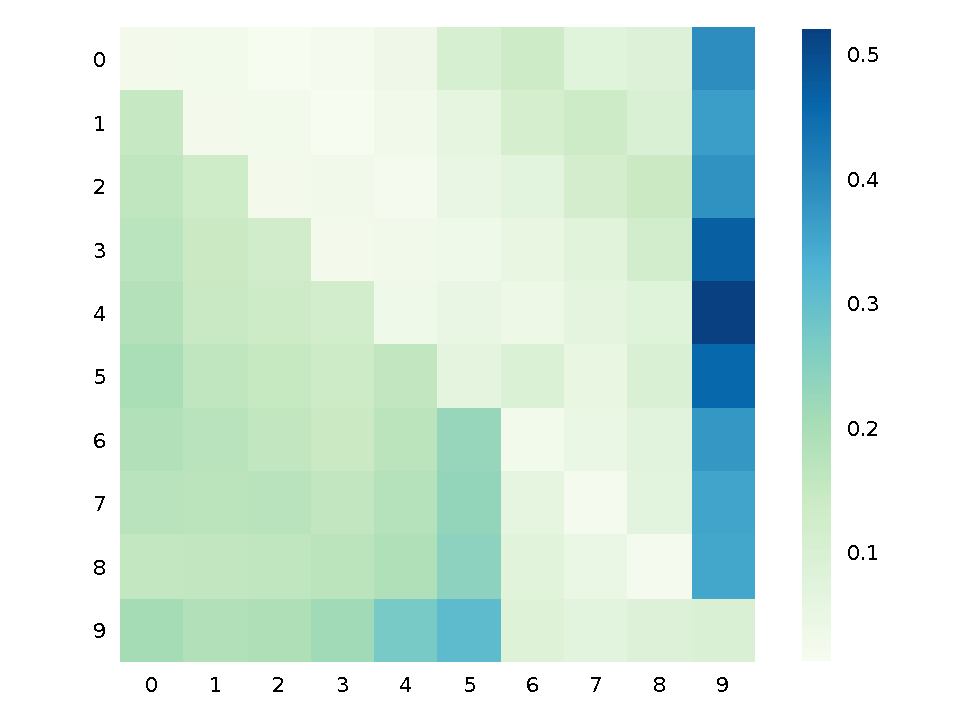
\includegraphics[width=\textwidth]{./figs/256_BERT_Attention_layer_0_head_1}
            \captionof{subfigure}{Layer 1, head 1}
            \end{minipage}
            \hfil
            \begin{minipage}{0.45\textwidth}
            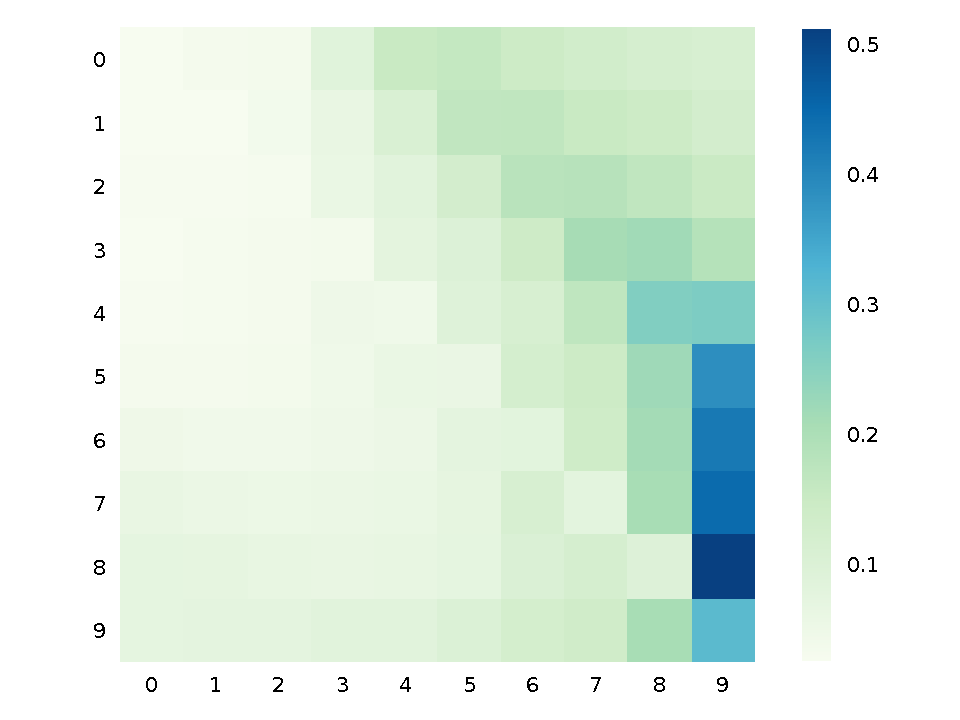
\includegraphics[width=\textwidth]{./figs/256_BERT_Attention_layer_0_head_2}
            \captionof{subfigure}{Layer 1, head 2}
            \end{minipage}
            
            \begin{minipage}{0.47\textwidth}
            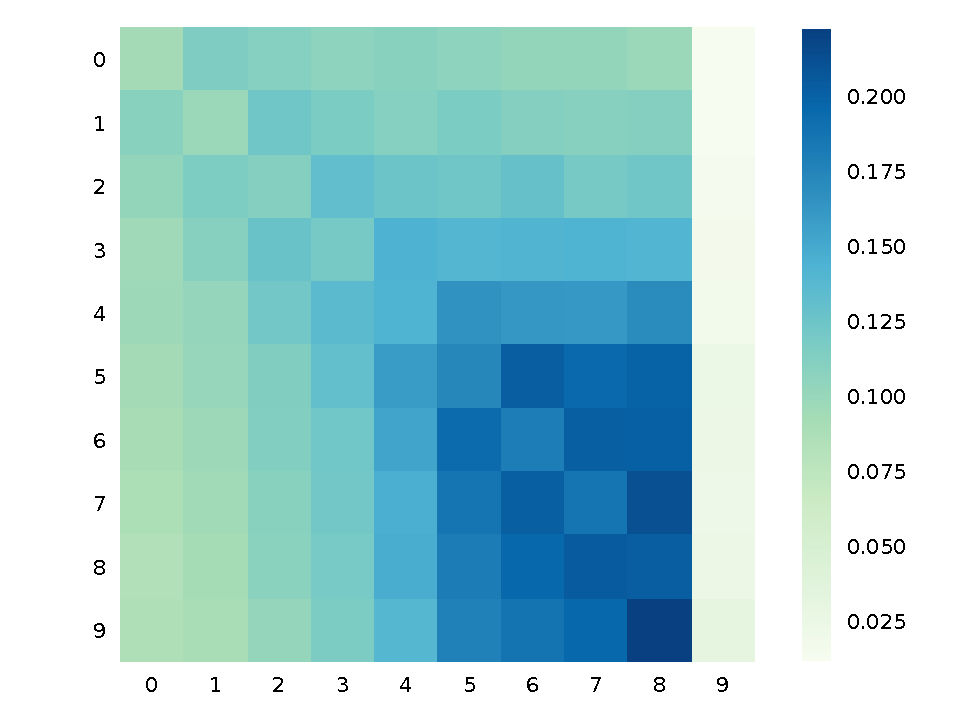
\includegraphics[width=\textwidth]{./figs/256_BERT_Attention_layer_1_head_2}
            \captionof{subfigure}{Layer 2, head 2}
            \end{minipage}
            \hfil
            \begin{minipage}{0.47\textwidth}
            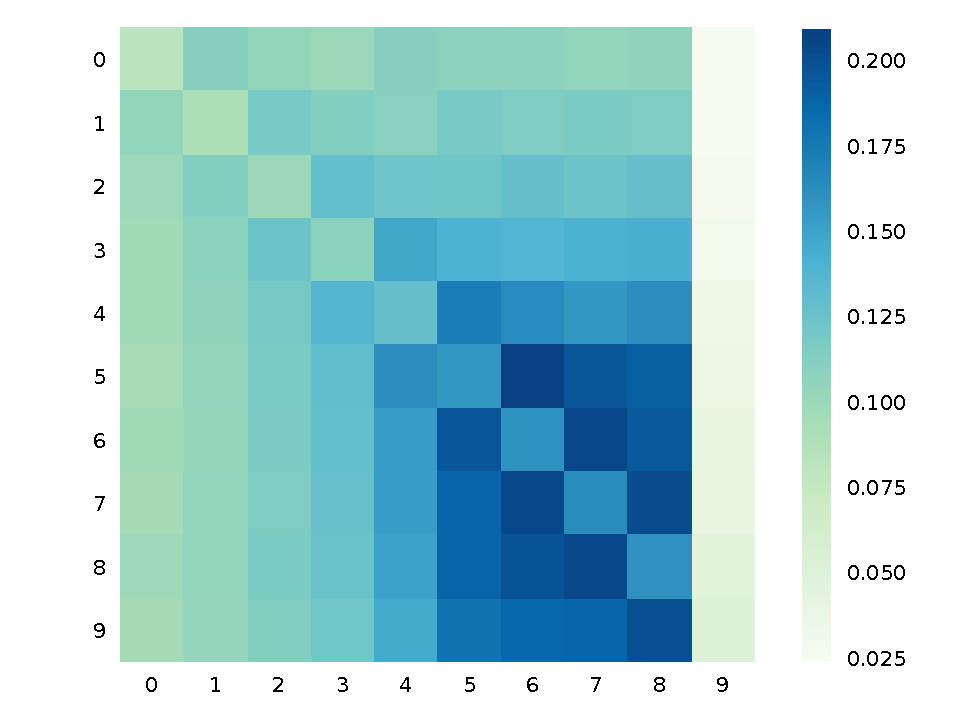
\includegraphics[width=\textwidth]{./figs/256_BERT_Attention_layer_1_head_4}
            \captionof{subfigure}{Layer 2, head 4}
            \end{minipage}
%            \captionof{figure}{caption}
        \end{tikzfigure}
%        \small \textbf{Heat-maps of average attention weights on Beauty, the last position ``9'' denotes ``\texttt{[mask]}'' (best viewed in color).}
        \centering
        \parbox{0.9\linewidth}{\bfseries \small Heat-maps of average attention weights on Beauty, the last position ``9'' denotes ``\texttt{[mask]}'' (best viewed in color).}
        
        \vspace*{0.5cm}
        \normalsize 
        \begin{itemize} [leftmargin=1.6cm]
            \item Attention varies across different heads.
            \item Attention varies across different layers.
            \item Items tend to attend on the items at both sides.
        \end{itemize}
        \end{minipage}
        }
    
    \block[linewidth=0pt, roundedcorners=0, bodyinnersep=15mm, bodyoffsetx=-2.5cm, bodyverticalshift=-0.9cm]{}{
    \centering
        \begin{minipage}{0.9\linewidth}
            {\Large \textbf{Ablation Study} }
        \vspace*{0.5cm}
        \normalsize
        \begin{center}
        \renewcommand{\arraystretch}{1.2}
        \setlength{\tabcolsep}{0.7em}
        \small
        \begin{tabular}{l r r r r}\toprule
         \multirow{2}{*}{Architecture} & \multicolumn{4}{c}{Dataset} \\ 
             \cmidrule(lr){2-5}
              & \multicolumn{1}{c}{Beauty} & \multicolumn{1}{c}{Steam} & \multicolumn{1}{c}{ML-1m} & \multicolumn{1}{c}{ML-20m} \\ \midrule
            $L=2$, $h=2$  & 0.1832 & 0.2241 & 0.4759 & 0.4513 \\ \midrule
            w/o PE  & 0.1741 & 0.2060 & 0.2155$\downarrow$ & 0.2867$\downarrow$ \\
            w/o PFFN  & 0.1803 & 0.2137 & 0.4544 & 0.4296 \\ \midrule
            w/o LN  & 0.1642$\downarrow$ & 0.2058 & 0.4334 & 0.4186 \\
            w/o RC  & 0.1619$\downarrow$ & 0.2193 & 0.4643 & 0.4483 \\
            w/o Dropout  & 0.1658 & 0.2185 & 0.4553 & 0.4471 \\ \midrule
            1 layer \hfill ($L=1$) & 0.1782 & 0.2122 & 0.4412 & 0.4238 \\
            3 layers \hfill ($L=3$) & \textbf{0.1859} & \textbf{0.2262} & \textbf{0.4864} & \textbf{0.4661}\\
            4 layers \hfill ($L=4$) & \textbf{0.1834} & \textbf{0.2279} & \textbf{0.4898} & \textbf{0.4732}\\ \midrule
            1 head \hfill($h=1$) & \textbf{0.1853} & 0.2187 & 0.4568 & 0.4402 \\
            4 heads \hfill ($h=4$) & 0.1830 & \textbf{0.2245} & \textbf{0.4770} & \textbf{0.4520} \\
            8 heads \hfill ($h=8$) & 0.1823 & \textbf{0.2248} & 0.4743 & \textbf{0.4550} \\
            \bottomrule
        \end{tabular}
        \end{center}
        \end{minipage}
        }

    
%    \block[linewidth=0pt, roundedcorners=0, bodyinnersep=15mm, bodyoffsetx=-2.5cm]{}{
%    \centering
%    \begin{minipage}{0.9\linewidth}
%        
%    \end{minipage}

%    }


\end{columns}


\block[linewidth=0pt, roundedcorners=0, bodyinnersep=68mm]{}{


}

%\colorlet{blockbodybgcolor}{regal_blue}
%     
%\block[linewidth=0pt, roundedcorners=0, bodyinnersep=18mm]{}{
%\color{white}
%\qrcode[hyperlink,height=2in]{http://ofey.me/projects/wordrep/}
%}

\node [above right, text centered,
       outer sep=0pt,
       minimum width=\paperwidth,
       minimum height=9cm,
       align=left, font=\huge,
       fill=regal_blue] (footer)
at (bottomleft) 
{
\begin{minipage}{0.15\linewidth}
\color{white} 
\qrcode[hyperlink,height=2in]{https://github.com/FeiSun/BERT4Rec} 
\end{minipage}
\hspace{-8cm}
\begin{minipage}{0.1\linewidth}
    \color{white} 
%\vspace{0.5cm}
\centering
{\fontsize{140}{140} \selectfont \faMobilePhone} 

\Large
Scan it!
\end{minipage}

\begin{minipage}{0.35\linewidth}
\vspace*{1cm}
\centering
~~~~~~~~~
\includegraphics[scale=0.5]{cikm_logo.png}
\end{minipage}
\hspace{8cm}
\begin{minipage}{0.25\linewidth}
    
\includegraphics[scale=1.6]{Alibaba_logo}
\end{minipage}

};


\draw [-, line width=2mm, regal_blue] ($(main.south)+(15, 0)$) to ($(main.south)+(15,-80)$);

%\node [above right, 
%       outer sep=0pt, font=\Large,
%       minimum width=\paperwidth,
%       minimum height=9cm,
%       align=right]
%at (bottomleft) 
%{\begin{minipage}{0.4\linewidth}
%    \color{white} 
%\centering
%{\fontsize{140}{140} \selectfont \faMobilePhone} 
%
%Scan it!
%\end{minipage}
%\begin{minipage}{0.4\linewidth}
%
\includegraphics[scale=1.6]{Alibaba_logo}
%\end{minipage}
%\hspace{10cm}
%};

%\node [above right, 
%       outer sep=0pt,
%       minimum width=\paperwidth,
%       minimum height=9cm,
%       align=right]
%at (bottomleft) 
%{
%\hspace{55cm}
\includegraphics[scale=1.6]{Alibaba_logo}
%};

\end{document}

